		Following the approach in \probref{prob:12/11/3/9/plane},
		the desired equation is 
\begin{align}
\myvec{	1&-7}\vec{x} -5
+
	k\myvec{3&1} \vec{x} = 0
	\\
	\implies 
	\myvec{	1 + 3k&-7+k} 
	 \vec{x} =5 
	 \\
	 \implies 
	\myvec{	1 + 3k \\ -7+k}  = \alpha \myvec{1 \\ 0}
	\text{or, } k = 7, \alpha =  22.
\end{align}
The desired equation is then given by 
\begin{align}
	\myvec{1&0}\vec{x}=\frac{5}{22}
\end{align}
See  
\figref{fig:chapters/11/10/4/6/Fig3}.
\begin{figure}[H]
  \begin{center} 
      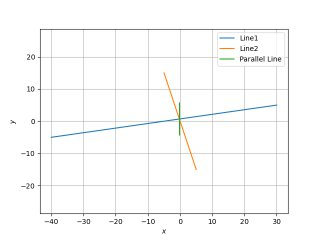
\includegraphics[width=0.75\columnwidth]{chapters/11/10/4/6/figs/line_fig.png}
  \end{center}
\caption{}
\label{fig:chapters/11/10/4/6/Fig3}
\end{figure}
